\documentclass[11pt]{article} 
\usepackage[english]{babel}
\usepackage[utf8]{inputenc}
\usepackage[margin=0.5in]{geometry}
\usepackage{amsmath}
\usepackage{amsthm}
\usepackage{amsfonts}
\usepackage{amssymb}
\usepackage[usenames,dvipsnames]{xcolor}
\usepackage{graphicx}
\usepackage[siunitx]{circuitikz}
\usepackage{tikz}
\usetikzlibrary{calc,arrows.meta}
\usepackage[colorinlistoftodos, color=orange!50]{todonotes}
\usepackage{hyperref}
\usepackage[numbers, square]{natbib}
\usepackage{fancybox}
\usepackage{epsfig}
\usepackage{soul}
\usepackage[framemethod=tikz]{mdframed}
\usepackage[shortlabels]{enumitem}
\usepackage[version=4]{mhchem}
\usepackage{multicol}
\usepackage{mathtools}
\usepackage{comment}
\usepackage{enumitem}
\usepackage[utf8]{inputenc}
\usepackage{listings}
\usepackage{color}
\usepackage[numbers]{natbib}
\usepackage{subfiles}
\usepackage{tkz-berge}
\usepackage{algorithm}
\usepackage[noend]{algpseudocode}


\newtheorem{prop}{Proposition}[section]
\newtheorem{thm}{Theorem}[section]
\newtheorem{lemma}{Lemma}[section]
\newtheorem{cor}{Corollary}[prop]

\theoremstyle{definition}
\newtheorem{definition}{Definition}

\theoremstyle{definition}
\newtheorem{required}{Problem}

\theoremstyle{definition}
\newtheorem{ex}{Example}

\tikzset{
	vertex/.style={circle,draw,minimum size=16, inner sep=0pt,font=\normalsize},
	every node/.style={draw=none,rectangle,font=\scriptsize,outer sep=0pt,inner sep=2pt},
	directed/.style={arrows={-Stealth[length=7pt]},font=\small},
	caption/.style={text width=6cm,align=center,rectangle,draw}
}


\setlength{\marginparwidth}{3.4cm}
%#########################################################

%To use symbols for footnotes
\renewcommand*{\thefootnote}{\fnsymbol{footnote}}
%To change footnotes back to numbers uncomment the following line
%\renewcommand*{\thefootnote}{\arabic{footnote}}

% Enable this command to adjust line spacing for inline math equations.
% \everymath{\displaystyle}

% _______ _____ _______ _      ______ 
%|__   __|_   _|__   __| |    |  ____|
%   | |    | |    | |  | |    | |__   
%   | |    | |    | |  | |    |  __|  
%   | |   _| |_   | |  | |____| |____ 
%   |_|  |_____|  |_|  |______|______|
%%%%%%%%%%%%%%%%%%%%%%%%%%%%%%%%%%%%%%%

\title{
\normalfont \normalsize 
\textsc{CSCI 3104 Fall 2021 \\ 
Instructors: Profs. Grochow and Waggoner} \\
[10pt] 
\rule{\linewidth}{0.5pt} \\[6pt] 
\huge Midterm 2- Standard 23 \\
\rule{\linewidth}{2pt}  \\[10pt]
}
%\author{Your Name}
\date{}

\begin{document}
\definecolor {processblue}{cmyk}{0.96,0,0,0}
\definecolor{processred}{rgb}{200, 0, 0}
\definecolor{processgreen}{rgb}{0, 255, 0}
\DeclareGraphicsExtensions{.png}
\DeclareGraphicsExtensions{.gif}
\DeclareGraphicsExtensions{.jpg}

\maketitle


%%%%%%%%%%%%%%%%%%%%%%%%%
%%%%%%%%%%%%%%%%%%%%%%%%%%
%%%%%%%%%%FILL IN YOUR NAME%%%%%%%
%%%%%%%%%%AND STUDENT ID%%%%%%%%
%%%%%%%%%%%%%%%%%%%%%%%%%%
\noindent
Due Date \dotfill TODO \\
Name \dotfill \textbf{Didi Trifonova} \\
Student ID \dotfill \textbf{109388776} \\


\tableofcontents

\section{Instructions}
 \begin{itemize}
	\item The solutions \textbf{should be typed}, using proper mathematical notation. We cannot accept hand-written solutions. \href{http://ece.uprm.edu/~caceros/latex/introduction.pdf}{Here's a short intro to \LaTeX.}
	\item You should submit your work through the \textbf{class Canvas page} only. Please submit one PDF file, compiled using this \LaTeX \ template.
	\item You may not need a full page for your solutions; pagebreaks are there to help Gradescope automatically find where each problem is. Even if you do not attempt every problem, please submit this document with no fewer pages than the blank template (or Gradescope has issues with it).

	\item You \textbf{may not collaborate with other students}. \textbf{Copying from any source is an Honor Code violation. Furthermore, all submissions must be in your own words and reflect your understanding of the material.} If there is any confusion about this policy, it is your responsibility to clarify before the due date. 

	\item Posting to \textbf{any} service including, but not limited to Chegg, Discord, Reddit, StackExchange, etc., for help on an assignment is a violation of the Honor Code.

	\item You \textbf{must} virtually sign the Honor Code (see Section \ref{HonorCode}). Failure to do so will result in your assignment not being graded.
\end{itemize}


\section{Honor Code (Make Sure to Virtually Sign)} \label{HonorCode}

\begin{required}
\noindent 
\begin{itemize}
\item My submission is in my own words and reflects my understanding of the material.
\item I have not collaborated with any other person.
\item I have not posted to external services including, but not limited to Chegg, Discord, Reddit, StackExchange, etc.
\item I have neither copied nor provided others solutions they can copy.
\end{itemize}

%\noindent In the specified region below, clearly indicate that you have upheld the Honor Code. Then type your name. 
\end{required}

\begin{proof}[Agreed (Didi Trifonova).] \\
I agree to the above
\end{proof}



\newpage
\section{Standard 23- DP: Use Recurrence to Solve}
\begin{required}
The \textsf{Subset-Sum} problem is defined as follows.
\begin{itemize}
\item \textsf{Instance:} We are given $n$ items with positive weights $w_{1}, \ldots, w_{n} > 0$, as well as a target threshold $W > 0$.  

\item \textsf{Solution:} Is there a subsequence $w_{i_{1}}, \ldots, w_{i_{k}}$ such that:
\[
\sum_{j=1}^{k} w_{i_{j}} = W.
\]

\noindent That is, can we select a subsequence of items whose combined weights add to $W$?
\end{itemize}

\noindent \\ For example, consider the input array $A = [4, 15, 8, 16, 23, 42].$
If $w = 31$ then the answer is ``TRUE'' since there is a subsequence $[15,16]$ where the sum is equal to $15 + 16 = 31$.
However, if $w = 13$ then the answer is ``FALSE'' since no subsequence of $A$ has sum equal $13$.

The \textsf{Subset-Sum} problem satisfies the following recurrence. For $0 \leq \ell \leq n$, and $0 \leq q \leq W$, define $T[\ell,q]$ be to TRUE if and only if there exists a subsequence of the first $\ell$ elements $[w_1,\dotsc,w_\ell]$ that sum to $q$. Then we have:
	\begin{align*}
	T[\ell, q] = 
	\begin{cases}
	TRUE & q=0\\
	FALSE & \ell = 0 \text{ and } q > 0\\
	T[\ell-1, q] & \ell > 0 \text{ and } w_{\ell} > q\\
	T[\ell-1, q] \text{ OR } T[\ell-1, q-w_{\ell}] & \ell > 0 \text{ and } w_\ell \leq q
	\end{cases}
	\end{align*}
(Note that in the final case, ``OR'' is the Boolean OR operation.) \\

\noindent Consider $A = [2, 1, 5, 3]$ and $W = 6$. Design and fill in a lookup table for this problem. Include all pointers. Clearly indicate whether a solution exists; and if so, how to recover it from the lookup table.
\end{required}

\begin{proof}[Answer] $ $ \\ 
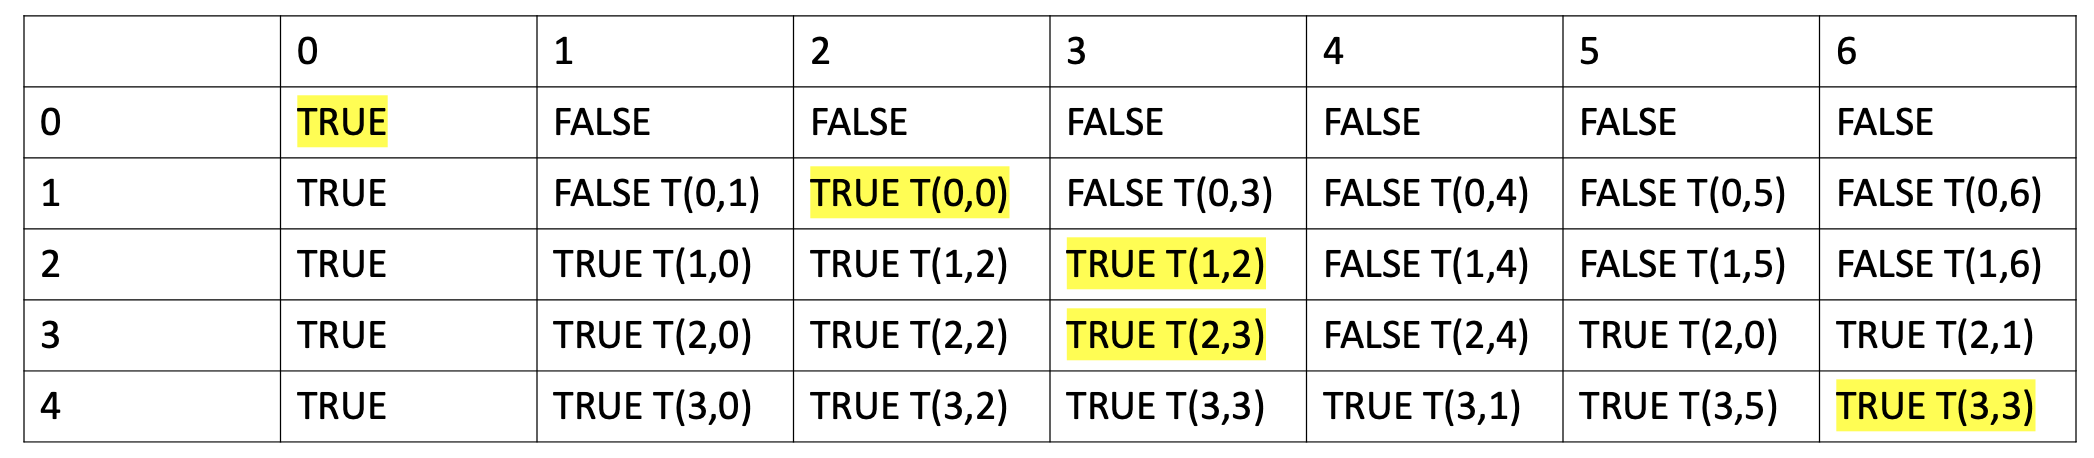
\includegraphics[width = 170 mm]{t1.png} \\
Yes, a solution does exist. The highlighted portions of the table show how we start at our final cell, T[4,6] and work our way back to T[0,0]. From T[1,2] we know our first item is $w_1$=2. Then we go to T[2,3] to get our second item, $w_2$=1. The next pointer is in the same column (same capacity) so we move on. Our last item is $w_4$=3 from cell T[4,6]. Our final subsequence is 2,1,3 and the total weight is 6, as desired. 
\end{proof}

%Include an Image: \includegraphics{ImageFileName}
%Include an Image and Rotate 90 degree: \includegraphics[angle=90]{ImageFileName}
%Include an Image, Rotate by 180 degrees, and scale by 50\% \includegraphics[scale=0.5, angle=90]{ImageFileName}



%%%%%%%%%%%%%%%%%%%%%%%%%%%%%%%%%%%%%%%%%%%%%%%%%%
\end{document} % NOTHING AFTER THIS LINE IS PART OF THE DOCUMENT



